\chapter{Cơ chế Attention cho mô hình Dịch máy}
\ifpdf
    \graphicspath{{Chapter3/Chapter3Figs/PNG/}{Chapter3/Chapter3Figs/PDF/}{Chapter3/Chapter3Figs/}}
\else
    \graphicspath{{Chapter3/Chapter3Figs/EPS/}{Chapter3/Chapter3Figs/}}
\fi
\label{chap_3}
\begin{quote}
\textit{Chương này trình bày về cơ chế Attention. Ở đây, chúng tôi tập trung tìm hiểu về các phiên bản của cơ chế Attention và đánh giá chúng dựa trên cơ sở Toán học. Cụ thể, chúng tôi tìm hiểu về hai phiên bản Toàn cục (Global) và Cục bộ (Local):
\begin{itemize}
	\item Toàn cục: chúng tôi nhận thấy sự hạn chế hiện có của kiến trúc Bộ mã hóa-Bộ mã hóa khi thực hiện dịch những câu dài. Do vậy, chúng tôi sử dụng cơ chế Attention phiên bản Toàn cục để giải quyết vấn đề này.
	\item Cục bộ: chúng tôi quan sát thấy rằng Attention Toàn cục vẫn còn một chút vấn đề về ý tưởng và chi phí tính toán. Với sự quan sát đó, chúng tôi hiệu chỉnh Attention Toàn cục thành phiên bản Attention Cục bộ để giải quyết những hạn chế đó.
\end{itemize}}
\end{quote}
\section{Cơ chế Attention}
Ở phần trước, chúng tôi đã trình bày về kiến trúc Bộ mã hóa-Bộ giải mã cùng với những điểm mạnh của nó trong việc giải quyết bài toán Dịch máy. Tuy nhiên, kiến trúc này vẫn còn tồn tại hạn chế về việc dịch những câu dài do những thông tin được mã hóa của câu nguồn bị mất dần theo các thời điểm về sau. Lí do mà vấn đề này tồn tại thực chất là bởi vì các mô hình LSTM được sử dụng trong Bộ mã hóa và Bộ giải mã. Bản thân mô hình LSTM chưa thật sự giải quyết hoàn toàn vấn đề "sự phụ thuộc dài hạn". Để có thể vẫn tận dụng được các mô hình LSTM mà vẫn nâng cao được chất lượng dịch, chúng tôi sử dụng cơ chế Attention.

Trước khi đi vào cách hoạt động của cơ chế Attention, chúng tôi điểm qua một chút về nguồn cảm hứng và lịch sử của cơ chế này. Cơ chế Attention được lấy cảm hứng trên cơ chế đặt sự chú ý khi quan sát sự vật, hiện tượng của thị giác con người. Khi con người quan sát một sự vật, hiện tượng nào đó bằng mắt, con người chỉ có thể tập trung vào một vùng nhất định trên sự vật, hiện tượng được quan sát để ghi nhận thông tin. Sau đó, khi cần ghi nhận thêm thông tin khác, con người sẽ di chuyển vùng tập trung lên vật thể của mắt sang vị trí khác. Những vùng lân cận xung quanh vùng tập trung sẽ bị "mờ" hơn so với vùng tập trung. Cơ chế Attention đã được ứng dụng trong lĩnh vực Thị giác máy tính từ khá lâu \cite{attentionhistory2010} \cite{attentionhistory2011}. Vào những năm gần đây, cơ chế Attention được sử dụng cho các kiến trúc mạng nơ-ron hồi quy trên bài toán Dịch máy và đã đạt được những kết quả ấn tượng.

\begin{figure}
	\centering
	\includegraphics[width=0.8\textwidth]{Attention-2}
	\caption[Minh họa cơ chế Attention.]{Minh họa cơ chế Attention. Một tầng Attention được đặt ở trước bước dự đoán đầu ra của bộ giải mã.}
	\label{fig_Attention}
\end{figure}
Cơ chế Attention được sử dụng trong đề tài này là một cơ chế sử dụng thông tin trong các trạng thái ẩn của RNN trong bộ mã hóa khi thực hiện quá trình giải mã. Cụ thể là:
\begin{itemize}
	\item Trong quá trình giải mã, trước khi dự đoán đầu ra, bộ giải mã nhìn vào các thông tin nằm trong các trạng thái ẩn của RNN ở bộ mã hóa.
	\item Ở mỗi phần tử đầu ra tại thời điểm $t$, bộ giải mã dựa vào trạng thái ẩn tại thời điểm $t$ hiện tại và quyết định sử dụng các thông tin trong trạng thái ẩn ở bộ mã hóa như thế nào.
\end{itemize}
2 phiên bản Toàn cục và Cục bộ mà trong khóa luận này chúng tôi trình bày là 2 cách mà cơ chế Attention sử dụng các trạng thái ẩn của RNN trong bộ mã hóa.
Để làm rõ hơn về ý tưởng của cơ chế Attention, dưới đây chúng tôi sẽ trình bày chi tiết về nền tảng Toán học của nó.
Attention sử dụng thêm một số đại lượng:
\begin{itemize}
	\item $a_t$: trọng số gióng hàng, $a_t$ được tính theo công thức dưới đây:
	\begin{equation}
	a_t = \text{align}(h_t, \bar{h}_s) = \frac{\exp\left(\text{score}(h_t, \bar{h}_s)\right)}{\sum_{s^{'}}\exp\left(\text{score}(h_t, \bar{h}_{s^{'}})\right)}
	\end{equation}
	$a_t$ là một véc-tơ chứa các điểm số giữa trạng thái ẩn ở thời điểm $t$ $h_t$ và các trạng thái ẩn ở câu nguồn $\bar{h}_s$. Hàm điểm số score mà chúng tôi sử dụng là gồm 2 hàm:
	\begin{equation}
	\text{score}(h_t, \bar{h}_s) = \left\{
			\begin{array}{ll}
			h^T_t\bar{h}_s \ \quad\quad dot\\
			h^T_tW_a\bar{h}_s	\quad general
			\end{array}
		\right.
	\end{equation}
	// TODO: Phân tích 2 hàm
	\item $c_t$: véc-tơ ngữ cảnh tại thời điểm $t$, là trung bình có trọng số của các trạng thái ẩn ở câu nguồn:
	\begin{equation}
	c_t = \sum_{s}a_{ts}h_s
	\end{equation}
	// TODO: Phân tích ý tưởng của véc-tơ ngữ cảnh. 
	\item $\tilde{h}_t$, véc-tơ attention tại thời điểm $t$, được tính như sau:
	\begin{equation}
	\boldsymbol{\tilde{h}_t} = \tanh(\bm{W_c}[\bm{c_t};\bm{h_t}])
	\end{equation}
\end{itemize}
Bước dự đoán đầu ra không thay đổi ngoài trạng thái ẩn $\bm{h_t}$ được thay thế bởi véc-tơ attention $\bm{\tilde{h}_t}$. $\bm{\tilde{h}_t}$ được đưa qua tầng softmax để cho ra phân bố xác suất dự đoán trên các từ:
\begin{equation}
p(y_t | y_{<t}, x) = \text{softmax}(\bm{W_s\tilde{h}})
\end{equation}
Nói một cách đơn giản, mục tiêu của cơ chế Attention là xoay quanh việc tìm véc-tơ ngữ cảnh $c_t$ một cách hiệu quả.
Tiếp theo, chúng tôi trình bày chi tiết hơn về 2 phiên bản Toàn cục và Cục bộ. 2 phiên bản này chỉ khác nhau về cách suy ra véc-tơ ngữ cảnh $\bm{c_t}$, còn các bước còn lại giống nhau.
Quy trình tính toán của cơ chế Attention: $h_t -> a_t -> c_t -> \tilde{h}_t$
\section{Attention Toàn cục}
Ý tưởng của Attention toàn cục là nhìn vào toàn bộ các vị trí nguồn (các trạng thái ẩn của RNN ở bộ mã hóa) khi thực hiện giải mã.
Khi đó trọng số gióng hàng $a_t$ là một véc-tơ có kích thước thay đổi và bằng số trạng thái ẩn (số từ) ở câu nguồn: $\text{len}(a_t) = S$.

\begin{equation}
a_t = \text{align}(h_t, \bar{h}_s) = \frac{\exp\left(\text{score}(h_t, \bar{h}_s)\right)}{\sum^{S}_{s^{'}=1}\exp\left(\text{score}(h_t, \bar{h}_{s^{'}})\right)}
\end{equation}

\begin{figure}
	\centering
	\includegraphics[width=0.8\textwidth]{Global-Attention_2.png}
	\caption[Minh họa cơ chế Attention Toàn cục.]{Minh họa cơ chế Attention Toàn cục. Tại thời điểm $t$, bộ giải mã nhìn vào toàn bộ các vị trí nguồn.}
	\label{fig_Global_Attention}
\end{figure}

Ưu điểm của phương pháp này là ý tưởng đơn giản, dễ cài đặt nhưng vẫn đạt được hiệu quả tốt (sẽ được trình bày ở phần thực nghiệm). Tuy nhiên, ý tưởng này vẫn còn chưa thực sự tự nhiên và còn hạn chế. Khi dịch một từ thì không cần phải đặt "sự chú ý" lên toàn bộ câu nguồn, chỉ cần đặt "sự chú ý" lên một số từ cần thiết. Mặc dù khi mô hình Attention Toàn cục được huấn luyện tốt thì hoàn toàn có thể chỉ đặt "sự chú ý" lên một số từ thật sự cần thiết, nhưng dễ thấy rằng bản thân mô hình vẫn phải tiêu tốn chi phí cho việc tính toán trọng số gióng hàng $a_t$ cho những vị trí không cần thiết. Đó là trường hợp lý tưởng cho mô hình Attention Toàn cục, nhưng trong thực tế, để đạt được độ chính xác như thế thì phải tiêu tốn nhiều tài nguyên cho việc huấn luyện mô hình như tài nguyên về tập dữ liệu đủ lớn, đủ tốt hay thời gian huấn luyện phải đủ lâu.
Để giải quyết hạn chế trên của Attention Toàn cục, chúng tôi đã tìm hiểu và sử dụng phiên bản tinh tế hơn, đó là mô hình Attention Cục bộ. Ở phần tiếp theo, chúng tôi sẽ trình bày về mô hình này.

\section{Attention Cục bộ}
Như đã nêu ở phần trước, Attention Toàn cục có một hạn chế là đặt "sự chú ý" lên toàn bộ các từ ở câu nguồn khi dịch từng từ ở câu đích. Điều này gây tiêu tốn chi phí tính toán và có thể tạo ra những câu dịch không thực tế khi dịch những câu dài như trong các đoạn văn hay trong một tài liệu. Attention Cục bộ ra đời để giải quyết hạn chế này.

Khi dịch mỗi từ ở câu đích, Attention Cục bộ chỉ đặt "sự chú ý" lên một số từ gần nhau ở câu nguồn. Mô hình này lấy cảm hứng từ sự đánh đổi giữa 2 mô hình "soft attention" và "hard attention" được đề xuất trong công trình Show, Attend and Tell \cite{showattendandtellXu2015} để giải quyết bài toán Phát sinh câu miêu tả cho ảnh (Image Captioning). Trong công trình \cite{showattendandtellXu2015}, Attention Toàn cục tương ứng với "soft attention", "sự chú ý" được đặt trên toàn bộ bức ảnh. Còn "hard attention" thì đặt "sự chú ý" lên một số phần của bức ảnh.

Dễ thấy, với cách hoạt động chỉ tập trung một số các từ gần nhau ở câu nguồn, mô hình hoạt động gần với cách con người tập trung vào một sự vật, hiện tượng nào đó. Chi phí cho huấn luyện và dự đoán sẽ được giảm bớt bởi vì chúng ta chỉ thực hiện tính véc-tơ trọng số gióng hàng $a_t$ cho những từ mà mô hình đặt "sự chú ý" lên.

Để làm rõ hơn về cách thức hoạt động của mô hình Attention Cục bộ, chúng tôi sẽ trình bày cụ thể hơn về nền tảng Toán học của mô hình này. Bên cạnh những đại lượng đã có ở mô hình Attention Toàn cục, Attention Cục bộ có thêm một số đại lượng như sau:
\begin{itemize}
	\item $p_t$: vị trí được gióng hàng.
\end{itemize}

\subsection{Thuật toán ``Sleep-Wake Stochastic Gradient Descent''}
Để khắc phục khó khăn của việc huấn luyện SRAEs với chuẩn L1, chúng tôi đề xuất một phiên bản điều chỉnh của thuật toán ``Stochastic Gradient Descent'' (SGD), gọi là ``Sleep-Wake Stochastic Gradient Descent'' (SW-SGD). Ý tưởng là trong mỗi ``epoch'' của SGD (một ``epoch'' ứng một lần duyệt qua tất cả các mẫu trong tập huấn luyện), ta tính tổng giá trị đầu ra của mỗi nơ-ron ẩn; và sau mỗi ``epoch'', ta kiểm xem có nơ-ron nào ``ngủ'' không (có tổng giá trị đầu ra bằng không) và ``đánh thức'' chúng bằng cách khởi tạo lại véc-tơ trọng số đi vào. Mặc dù cách làm này rất đơn giản, nhưng thí nghiệm của chúng tôi cho thấy nó có thể giúp SRAEs học được thành công các đặc trưng mà không có đặc trưng nào ``ngủ''.

Một cách cụ thể, cho tập huấn luyện không có nhãn $\{x^{(1)}, x^{(2)}, \ldots, x^{(N)}\}$, thuật toán SW-SGD dùng để cực tiểu hóa hàm chi phí sau của SRAEs:
\begin{equation}
\begin{split}
	C(W) &= \frac{1}{N}\sum_{i=1}^N C^{(i)}(W)\\
		 &= \frac{1}{N}\sum_{i=1}^N\left(\|x^{(i)} - \hat{x}^{(i)}\|_2^2 + \lambda \|h^{(i)}\|_1\right)
\end{split}
\end{equation}
Trong đó:
\begin{itemize}
	\item $h^{(i)}$ là véc-tơ đầu ra ở tầng ẩn tương ứng với véc-tơ đầu vào $x^{(i)}$: \[h^{(i)} = \max\left(0, W^{(e)}x^{(i)} + b^{(e)}\right)\]
	\item $\hat{x}^{(i)}$ là véc-tơ tái tạo của véc-tơ đầu vào $x^{(i)}$: \[\hat{x}^{(i)} = W^{(d)}h^{(i)} + b^{(d)}\]
	\item $W=\{W^{(e)}, b^{(e)}, W^{(d)}, b^{(d)}\}$ là các tham số của SRAEs.
\end{itemize}
Từng bước của thuật toán SW-SGD được trình bày ở thuật toán \ref{alg_SW-SGD} (những chỗ thay đổi so với thuật toán SGD ban đầu được \emph{in nghiêng}).
%\begin{leftbar}
%\begin{enumerate}
%	\item Khởi tạo ngẫu nhiên cho $W$.
%	\item Lặp cho đến khi thỏa điều kiện dừng:
%	\begin{itemize}
%		\item \emph{Khởi tạo véc-tơ $s$ gồm có $D_h$ phần tử (với $D_h$ là số lượng nơ-ron ẩn của SRAEs), trong đó mỗi phần tử có giá trị bằng $0$ (phần tử $s_j$ của véc-tơ $s$ dùng để lưu tổng giá trị đầu ra của nơ-ron ẩn $j$ với tất cả các mẫu trong tập huấn luyện sau một ``epoch'').}
%		\item Xáo trộn ngẫu nhiên thứ tự của các mẫu trong tập huấn luyện (thường sẽ giúp hội tụ nhanh hơn).
%		\item Với ``mini-batch'' thứ $b=1,2,\ldots,\frac{N}{B}$ ($N$ là số lượng mẫu trong tập huấn luyện, $B$ là kích thước của ``mini-batch''):
%		\begin{itemize}
%			\item Với mẫu huấn luyện thứ $i=(b-1)B+1, (b-1)B+2, \ldots, bB$:
%			\begin{itemize}
%				\item Lan truyền tiến với véc-tơ đầu vào $x^{(i)}$.
%				\item \emph{Cập nhật véc-tơ $s$: $s = s + h^{(i)}$ (với $h^{(i)}$ là véc-tơ đầu ra ở tầng ẩn tương ứng với véc-tơ đầu vào $x^{(i)}$).}
%				\item Lan truyền ngược và tính véc-tơ đạo hàm riêng $\nabla C^{(i)}(W)$.
%			\end{itemize}
%			\item Cập nhật $W$:
%			\[W = W - \alpha \frac{1}{B} \sum_{i=(b-1)B+1}^{bB} \nabla C^{(i)}(W)\]
%			($\alpha > 0$ là hệ số học)
%		\end{itemize}
%		\item \emph{Kiểm xem có nơ-ron ẩn nào ``ngủ'' (có tổng đầu ra $s_j=0$) và ``đánh thức'' bằng cách khởi tạo lại véc-tơ trọng số đi vào nơ-ron ẩn này.}
%	\end{itemize}
%\end{enumerate}
%\end{leftbar}
\begin{algorithm}
	\newalgname{Thuật toán}
	\caption{Sleep-Wake Stochastic Gradient Descent (SW-SGD)}
	\label{alg_SW-SGD}
	\begin{algorithmic}[1]
		\renewcommand{\algorithmicrequire}{\textbf{Đầu vào:}}
		\renewcommand{\algorithmicensure}{\textbf{Đầu ra:}}
		\algnewcommand\algorithmicoperation{\textbf{Thao tác:}}
		\algnewcommand\Operation{\item[\algorithmicoperation]}
		
		\Require Tập huấn luyện không có nhãn $\{x^{(1)},\ldots,x^{(N)}\}$, hệ số học $\alpha>0$, kích thước ``mini-batch'' B
		\Ensure Bộ tham số $W$ của SRAEs để cho hàm chi phí $C(W)$ đạt cực tiểu
		
		\Operation
		\State Khởi tạo ngẫu nhiên cho $W$
		\While{chưa thỏa điều kiện dừng} \%\% Với mỗi ``epoch''
			\State \parbox[t]{\dimexpr\linewidth-\algorithmicindent}{\emph{Khởi tạo véc-tơ $s$ gồm có $D_h$ phần tử (với $D_h$ là số lượng nơ-ron ẩn của SRAEs), trong đó mỗi phần tử có giá trị bằng $0$ (phần tử $s_j$ của véc-tơ $s$ dùng để lưu tổng giá trị đầu ra của nơ-ron ẩn $j$ với tất cả các mẫu trong tập huấn luyện sau một ``epoch'')}\strut}
			\State \parbox[t]{\dimexpr\linewidth-\algorithmicindent}{Xáo trộn ngẫu nhiên thứ tự của các mẫu trong tập huấn luyện (thường sẽ giúp hội tụ nhanh hơn)\strut}
			\For{b = 1 : N/B} \%\% Với mỗi ``mini-batch''
				\For{i = (b-1)B+1 : bB} \%\% Với mỗi mẫu huấn luyện trong ``mini-batch''
					\State Lan truyền tiến với véc-tơ đầu vào $x^{(i)}$
					\State \parbox[t]{\dimexpr\linewidth-\algorithmicindent}{\emph{Cập nhật véc-tơ $s$: $s = s + h^{(i)}$ \\(với $h^{(i)}$ là véc-tơ đầu ra ở tầng ẩn tương ứng với véc-tơ đầu vào $x^{(i)}$)}\strut}
					\State Lan truyền ngược và tính véc-tơ đạo hàm riêng $\nabla C^{(i)}(W)$
				\EndFor
				\State Cập nhật $W$: $W = W - \alpha \frac{1}{B} \sum_{i=(b-1)B+1}^{bB} \nabla C^{(i)}(W)$ 
			\EndFor
			\State \parbox[t]{\dimexpr\linewidth-\algorithmicindent}{\emph{Kiểm xem có nơ-ron ẩn nào ``ngủ'' (có tổng đầu ra $s_j=0$) và ``đánh thức'' bằng cách khởi tạo lại véc-tơ trọng số đi vào nơ-ron ẩn này}}
		\EndWhile
	\end{algorithmic}
\end{algorithm}

\section{Ràng buộc trọng số trong SRAEs}
Bên cạnh ràng buộc thưa, ràng buộc trọng số cũng là một thành phần quan trọng để làm cho SAEs ``hoạt động''. Tại sao cần phải ràng buộc trọng số? Ví dụ, trong Sparse Coding, ta cần phải ràng buộc các véc-tơ cơ sở được chuẩn hóa (có chiều dài bằng 1); nếu không thì sẽ xảy ra trường hợp là giá trị của hàm chi phí ở công thức (\ref{eq_SparseCoding}) có thể được làm giảm xuống một cách ``tầm thường'' bằng cách chia hệ số cho một số lớn tùy ý và nhân véc-tơ cơ sở tương ứng với cùng số lớn đó (làm như vậy sẽ làm độ thưa giảm xuống tùy ý, còn độ lỗi tái tạo thì giữ nguyên). Các véc-tơ cơ cở trong ``Sparse Coding'' tương ứng với các cột của ma trận trọng số $W^{(d)}$ của bộ giải mã của SAEs (mỗi cột của $W^{(d)}$ ứng với véc-tơ trọng số đi ra tại mỗi nơ-ron ẩn). Như vậy, trong SAEs, ta cũng có thể ràng buộc mỗi cột của $W^{(d)}$ được chuẩn hóa (có chiều dài bằng 1) giống như ở Sparse Coding. Nhưng còn ma trận trọng số $W^{(e)}$ của bộ mã hóa của SAEs? Ta nên ràng buộc $W^{(e)}$ như thế nào cho hợp lý?

Dưới đây là một số cách đã được đề xuất để ràng buộc trọng số của SAEs:
\begin{itemize}
	\item \textbf{Ràng buộc $W^{(d)} = (W^{(e)})^T$}: bộ trọng số được dùng chung cho cả bộ mã hóa và bộ giải mã (cụ thể là $W^{(d)}$ và $W^{(e)}$ là chuyển vị của nhau) \cite{coates2012demystifying}. Cách ràng buộc trọng số này cũng được dùng trong các loại ``Auto-Encoders'' khác như ``Denoising Auto-Encoders'' và ``Contractive Auto-Encoders'' \cite{vincent2008extracting}\cite{rifai2011contractive}\cite{rifai2011HCAEs}. Lưu ý là tất cả \cite{coates2012demystifying}\cite{vincent2008extracting}\cite{rifai2011contractive}\cite{rifai2011HCAEs} đều dùng hàm kích hoạt sigmoid ở tầng ẩn. Trong trường hợp dùng hàm kích hoạt tuyến tính ($f(x) = x$) ở tầng ẩn, ràng buộc $W^{(d)} = (W^{(e)})^T$ sẽ có xu hướng làm cho các véc-tơ cơ sở (các dòng của $W^{(e)}$ hay các cột của $W^{(d)}$) trực giao với nhau và được chuẩn hóa \cite{le2011ica}; nhưng trong trường hợp dùng hàm kích hoạt sigmoid ở tầng ẩn, ta không rõ chuyện gì đang xảy ra. Một điểm lợi của việc dùng chung bộ trọng số là tiết kiệm bộ nhớ lưu trữ; điều này sẽ có ích khi cài đặt song song trên GPU (Graphical Processing Units).
	\item \textbf{Ràng buộc $W^{(d)}$ được chuẩn hóa}: các cột của $W^{(d)}$ được ràng buộc là có độ dài bằng 1 \cite{zeiler2013rectified}. Ràng buộc này tương tự như ở ``Sparse Coding'' và giúp ngăn chặn việc hàm chi phí có thể bị làm giảm xuống một cách ``tầm thường'' như đã nói ở trên. Nhưng còn bộ trọng số $W^{(e)}$ của bộ mã hóa? Chẳng hạn, để công bằng giữa các đặc trưng, ta cũng nên ràng buộc các véc-tơ dòng của $W^{(e)}$ (ứng với các véc-tơ trọng số đi vào các nơ-ron ẩn; các véc-tơ này đóng vai trò như các bộ lọc đặc trưng) có cùng độ dài.
	\item \textbf{Ràng buộc các trọng số có giá trị bình phương nhỏ (weight decay)}: các trọng số của cả bộ mã hóa và bộ giải mã đều được ràng buộc là có độ lớn nhỏ bằng cách phạt tổng bình phương của chúng \cite{goodfellow2009measuring}\cite{coates2011analysis}. Cách ràng buộc này vốn ban đầu được dùng trong mạng nơ-ron học có giám sát để tránh vấn đề quá khớp. Khi áp dụng cho SAEs, ta có hiểu nó là một phiên bản ``mềm'' của cách ràng buộc $W^{(d)}$ được chuẩn hóa ở trên và nhờ đó cũng sẽ giúp cho SAEs tránh khỏi tình trạng hàm chi phí bị giảm xuống một cách ``tầm thường''; ngoài ra, nó còn ràng buộc thêm là các véc-tơ dòng của $W^{(e)}$ (ứng với các bộ lọc đặc trưng) có độ dài xấp xỉ bằng nhau (đều nhỏ). Tuy nhiên, cách ràng buộc này lại làm xuất hiện thêm một siêu tham số; ta không muốn điều này.
\end{itemize}

\subsection{Cách ràng buộc trọng số đề xuất cho SRAEs}
Với SRAEs (SAEs sử dụng hàm kích hoạt ``rectified linear'' ở tầng ẩn), không rõ là ta nên sử dụng cách ràng buộc trọng số nào trong những cách ở trên. Trong phần này, chúng tôi đề xuất một cách ràng buộc trọng số mới và hợp lý cho SRAEs. Cách ràng buộc này không đưa thêm siêu tham số nào. Cụ thể là, cách ràng buộc trọng số của chúng tôi bao gồm đồng thời hai ràng buộc:
\begin{itemize}
	\item Thứ nhất, chúng tôi ràng buộc ma trận trọng số $W^{(e)}$ của bộ mã hóa và ma trận trọng số $W^{(d)}$ của bộ giải mã là chuyển vị của nhau: $W^{(d)} = (W^{(e)})^T$.
	\item Thứ hai, chúng tôi đồng thời cũng ràng buộc là các véc-tơ dòng của $W^{(e)}$ và các véc-tơ cột của $W^{(d)}$ được chuẩn hóa (có độ dài bằng 1). Ở đây, mỗi véc-tơ dòng của $W^{(e)}$ ứng với véc-tơ trọng số đi vào ở mỗi nơ-ron ẩn, và mỗi véc-tơ cột của $W^{(d)}$ ứng với véc-tơ trọng số đi ra ở mỗi nơ-ron ẩn.
\end{itemize}

Với một véc-tơ đầu vào $x$, nếu ta chỉ chú ý đến các nơ-ron được ``bật'' (có giá trị đầu ra khác không) ở tầng ẩn thì đây là một hệ thống tuyến tính (minh họa ở hình \ref{fig_SRAE}). Do đó, với hai ràng buộc ở trên, SRAEs sẽ chiếu véc-tơ đầu vào $x$ xuống một hệ trục tọa độ cục bộ sao cho từ hệ trục tọa độ này có thể tái tạo được tốt véc-tơ $x$ ban đầu; hệ trục tọa độ cục bộ này bao gồm một số ít các véc-tơ cơ sở (đã được chuẩn hóa) được chọn lựa bởi hàm ``rectified linear'' từ tập lớn các véc-tơ cơ sở. Ta có thể hiểu tập con các véc-tơ cơ sở này biểu diễn vùng không gian PCA cục bộ xung quanh $x$. Như vậy, SRAEs (với ràng buộc trọng số đề xuất của chúng tôi) có thể học được mặt phi tuyến mà ở đó dữ liệu tập trung bằng cách ghép nhiều mặt tuyến tính cục bộ lại với nhau (minh họa ở hình \ref{fig_local_charts}). Mỗi mặt tuyến tính cục bộ được phụ trách bởi một tập con các véc-tơ cơ sở. Điểm lợi ở đây là các véc-tơ cơ sở có thể được dùng chung giữa các mặt tuyến tính cục bộ láng giềng nhau.

\begin{figure}
	\centering
	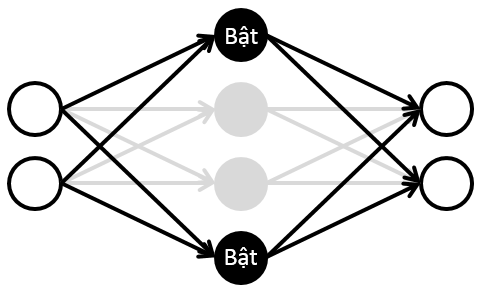
\includegraphics[width=0.6\textwidth]{SRAE}
	\caption[Minh họa SRAEs]{Minh họa SRAEs. Với một véc-tơ đầu vào, nếu ta chỉ chú ý đến các nơ-ron được ``bật'' (có giá trị đầu ra khác không) ở tầng ẩn thì đây là một hệ thống tuyến tính.}
	\label{fig_SRAE}
\end{figure}
\begin{figure}
	\centering
	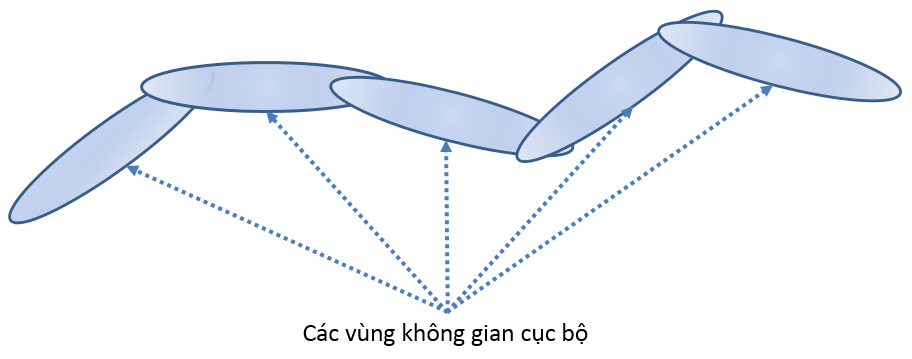
\includegraphics[width=\textwidth]{local_charts}
	\caption[Minh họa mặt phi tuyến mà SRAEs học được]{Với một véc-tơ đầu vào $x$, chỉ có một tập con các nơ-ron ẩn được bật. Tập con các véc-tơ cơ sở tương ứng với tập con các nơ-ron ẩn này biễu diễn một vùng không gian cục bộ xung quanh $x$ (giống như vùng không gian PCA cục bộ). Như vậy, SRAEs (với ràng buộc trọng số đề xuất của chúng tôi) có thể học được mặt phi tuyến mà ở đó dữ liệu tập trung bằng cách ghép nhiều mặt tuyến tính cục bộ lại với nhau. Mỗi mặt tuyến tính cục bộ được phụ trách bởi một tập con các véc-tơ cơ sở. Điểm lợi ở đây là các véc-tơ cơ sở có thể được dùng chung giữa các mặt tuyến tính cục bộ láng giềng nhau.}
	\label{fig_local_charts}
\end{figure}

Như vậy, ta cần phải tối thiểu hóa hàm chi phí của SRAEs với hai ràng buộc trọng số ở trên. Trong khi ràng buộc thứ nhất ($W^{(d)} = (W^{(e)})^T$) có thể được tích hợp dễ dàng vào thuật toán tối ưu hóa ``Stochastic Gradient Descent''  (SGD), ràng buộc thứ hai (các dòng của $W^{(e)}$ và các cột của $W^{(d)}$ được chuẩn hóa) thoạt nhìn khó có thể tích hợp vào thuật toán SGD và có thể ta cần phải sử dụng đến các phương pháp tối ưu hóa phức tạp hơn. Để giải quyết vấn đề này, chúng tôi thay đổi công thức lan truyền tiến của SRAEs như sau:
\begin{equation}
	h = \max(0, \hat{W}^{(e)}x + b^{(e)})
\end{equation}
\begin{equation}
	\hat{x} = (\hat{W}^{(e)})^Th + b^{(d)}
\end{equation}
Trong đó, ma trận $\hat{W}^{(e)}$ là ma trận $W^{(e)}$ với các dòng đã được chuẩn hóa (bằng cách lấy mỗi phần tử trên một dòng của $W^{(e)}$ chia cho căn bậc hai của tổng bình phương của tất cả các phần tử trên dòng đó). Ở đây, các tham số được học vẫn là $W^{(e)}$, $b^{(e)}$, và $b^{(d)}$. Bằng cách này, ta vẫn có thể sử dụng thuật toán SGD như bình thường. Khi đưa thêm bước chuẩn hóa vào công thức lan truyền tiến như vậy, ta cũng cần phải tính lại các đạo hàm riêng của hàm chi phí theo các tham số (sẽ phức tạp hơn so với công thức lan truyền tiến ban đầu). Chúng tôi sử dụng ngôn ngữ lập trình là Theano \cite{bergstra+al:2010-scipy}; nhờ tính năng tính đạo hàm một cách tự động của Theano, ở đây ta sẽ không cần phải tính toán cụ thể công thức của các đạo hàm riêng này.
